% !TEX root = ../agglo_clust_review.tex
% 

\begin{figure}
\centering
        \begin{subfigure}[t]{0.49 \textwidth}
        \centering
        \includegraphics[width=\textwidth,trim=0.55in 0.35in 0.65in 0.80in,clip]{./figs/merge_noise_only_direct.pdf}

        \caption{Without long-range edges: $p_{\mathrm{long}}=0$} \label{fig:merge_noise_only_direct}
    \end{subfigure} \hfill
    \begin{subfigure}[t]{0.49 \textwidth}
        \centering
        \includegraphics[width=\textwidth,trim=0.53in 0.35in 0.65in 0.80in,clip]{./figs/merge_noise_long_range.pdf}
        \caption{With long-range edges: $p_{\mathrm{long}}=0.1$} \label{fig:merge_noise_with_long_range}
    \end{subfigure}
\caption{Performances of \algname{} with different linkage criteria on a crop of CREMI training data sample B, depending on the amount of noise (x-axis) added to the CNN predictions. \textbf{Top}: Accuracy given by Rand-Score (higher is better). Solid lines represent median values. Values between the 25th and the 75th percentile are shown in shade areas. \textbf{Bottom}: Multicut objective (Eq. \ref{eq:multicut_obj}), measuring how balanced the final clusterings are (lower is better); for a clearer comparison, an offset is added to the energy values, so that the method achieving the lowest energy is always assigned to value 1. \UPDATE{CLC}  
}\label{fig:noise_plots}
\end{figure}

% \begin{minipage}[b]{0.48\textwidth}
% % \begin{figure}
%         % \begin{subfigure}[t]{0.48 \textwidth}
%         \centering
%         \includegraphics[width=0.98\textwidth,trim=0.35in 0.35in 0.35in 0.35in,clip]{./figs/merge_noise.pdf}

%         \captionof{subfigure}{Merge-biased opensimplex noise} \label{fig:thresh}
%     \end{minipage}\hfil
% \begin{minipage}[b]{0.48\textwidth}
%     % \end{subfigure}%
%     % \begin{subfigure}[t]{0.48 \textwidth}
%         \centering
%         \includegraphics[width=0.98\textwidth,trim=0.29in 0.31in 0.31in 0.31in,clip]{./figs/split_noise.pdf}
%         \captionof{subfigure}{Split-biased opensimplex noise} \label{fig:ws}
%     % \end{subfigure}
% \captionof{figure}{Plot illustrating Adapted RAND scores achieved by UGACA and different update rules when noise is added to the edge weights... Solid lines represent median values, whereas values between the 25th and the 75th percentile are shown in shade areas.    \TODO{Label which uses only local-neighbors and which uses long-range connections}}\label{fig:noise_plots}
% % \end{figure}



\subsection{In-depth comparison of different linkage criteria for \algname{}} \label{sec:comparison_exps}
As shown in Table \ref{tab:results_cremi_train}, among all the signed graph algorithms included in our generalized framework, the less-known one with \emph{Average} linkage consistently outperformed all other previously proposed linkage like \emph{Sum} or \emph{Absolute Max}. This method also achieved \UPDATE{comparable} scores to other complex multi-step pipelines that usually require the user to tune several hyper-parameters, like LMC. 
In Fig. \ref{fig:cremi_comparison}, we highlight some failure cases of \algname{} and in Appendix we provide an extended version of Table \ref{tab:results_cremi_train} including all linkage tested with \algname{} on the full CREMI training data. 

In order to highlight the properties and the strengths of each linkage criteria and  perform an in-depth comparison that is as quantitative as possible, we run an additional set of experiments where we perturbed the CNN predictions with noise. In Appendix, we provide all the details about the used type of spatially correlated noise that allowed us to perturb the CNN outputs by introducing simulated additional artifacts like missing or false boundary evidences (see visual example in Fig. \ref{fig:noisy_affs}).  

Plots in Fig. \ref{fig:noise_plots} summarize 6000 experiments: we focused on the best performing linkage criteria, i.e. \emph{Average}, \emph{Sum} and \emph{Abs Max}, and tested them with different values of noise, both with and without use of long-range connections in the grid-graph\footnote{We tested 20 values of noise and, for each setup, we averaged the scores over 30 runs.}. In Fig. \ref{fig:noise_plots}, we used a merge-biased noise decreasing boundary evidence. See Fig. \ref{fig:noise_split} in Appendix for a split-biased version. 
Our findings confirm that \algname{} with \emph{Average} linkage criterion represents the most robust algorithm tested and that is the one benefiting more from additional long-range edge connections. Other versions using cannot-link constraints generally lead to an over-segmentation, but are robust to ``leaks through holes'' given by missing boundary evidence. The greedy \emph{absolute maximum} linkage proposed by \cite{wolf2018mutex} is the least robust to noise, but, as we show in Table \ref{tab:full_cremi_results}, it represents an efficient and considerably faster option.   
The \emph{Sum} linkage generally outputs the most balanced graph partitioning according to the objective defined in Eq. \ref{eq:multicut_obj} and is then confirmed to be a good choice for initializing more complex approximations of the multicut optimization problem like \cite{beier2016efficient}. Nevertheless, in more challenging parts of the data (see Fig. \ref{fig:cremi_comparison}) or in the presence of noise, it often incorrectly merge regions together, leading to more unbalanced graph partitioning. In these cases, the use of cannot-link constraints or a more robust average linkage are preferable.  
% \UPDATE{The plots in Fig. \ref{fig:noise_plots} represent the scores achieved by \algname{} with different update rules depending on the amount of noise $\m{}athcal{K}$ added to the edge weights and the probability $p_{\mathrm{long}}$ of long-range connections in the graph. Results clearly show that adding long-range edges is always beneficial for the final segmentation \TODO{Not True!}. \TODO{What about time?} The most robust version of update rule proved to be the \emph{mean}, that achieves similar scores even with significantly noisy edge weights. The \emph{absolute maximum} update rule proposed by \cite{wolf2018mutex} provides an efficient and fast option, but completely fails when too much noise is added. 
% The \emph{sum} update rule version was the slowest option tested, but it was not as robust as the \emph{mean} version, probably due to its tendency to grow one cluster at the time (see Sec. \ref{sec:exp_first_comparison}). \TODO{Comment about MC energy}
% On the other hand, \algname{} with \emph{mean} update rule and cannot-link constraints did not achieve high scores because of the strong over-segmentation error.}


% Highlight difference of the sum in Fig. \ref{fig:intro_figure}.
% \begin{itemize}
%   % \item compare different choices of signed-cost-mappings (say which one worked best)
%   % \item present cremi crop-C table and rule out single and complete linkage
% \end{itemize}




\begin{figure}[b]
\centering
\begin{minipage}[T]{0.54\textwidth}
    \centering
    \footnotesize
        \begin{tabular}{l|l|cc}
           & \algname{}  &  \multicolumn{2}{c}{Use constraints:} \\
           & Linkage & \textsc{No} & \textsc{Yes} \\ \midrule
DWT \cite{bai2017deep} & - & 21.2 & - \\
SGN \cite{liu2017sgn} & - & 29.2 & - \\
Mask RCNN \cite{he2017mask} & - & 31.5 & - \\ \hline
 & \textbf{Average}& \textbf{34.3}  & 33.9  \\
 & GMIS-Agglo \cite{liu2018affinity} & \UPDATE{33.0} & -  \\
\multirow{2}{*}{GMIS Pipeline} & Max &   24.3  &   32.5  \\
 & Abs. Max. \cite{wolf2018mutex}  & 32.1 & 32.1 \\
 & Sum \cite{keuper2015efficient,levinkov2017comparative} & 31.3  & 31.9  \\
 & Min &  0    & 0  \\
        \end{tabular}
    \captionof{table}{AP scores on the cityscapes validation set for the generalized algorithm and different types of linkage criteria.  }
    \label{tab:results_cityscapes_val}
\end{minipage}\hfill
\begin{minipage}[T]{0.43\textwidth}
    \centering
    \centering
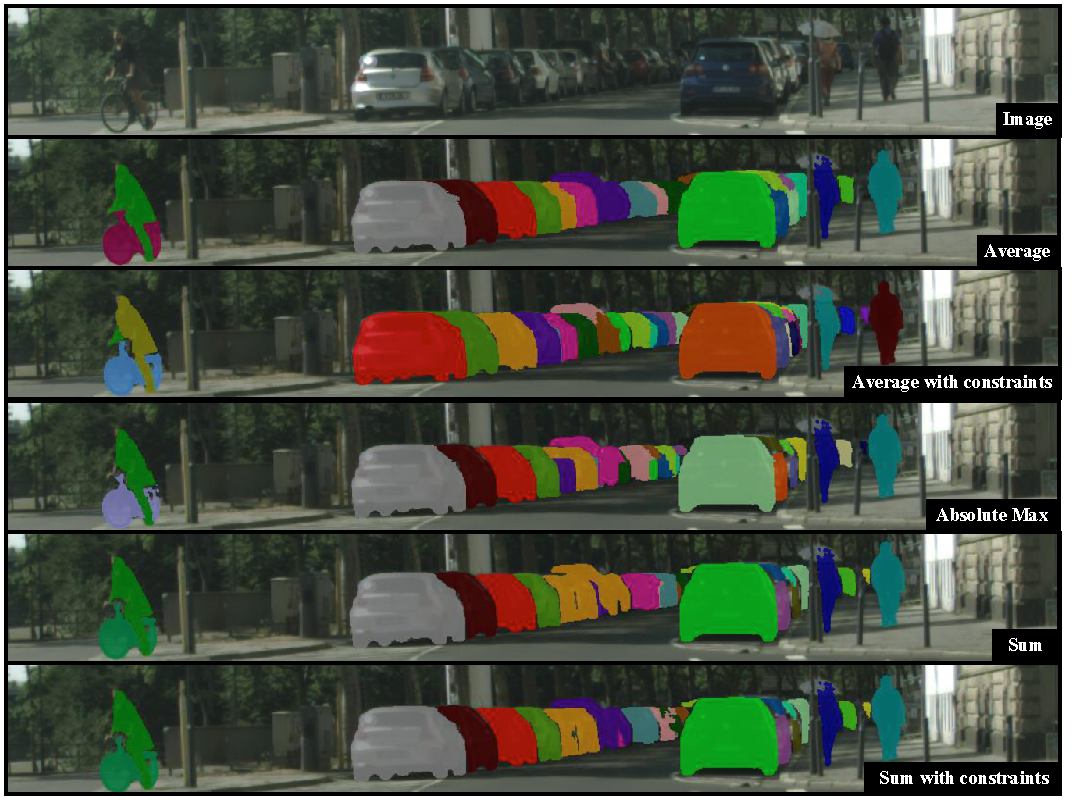
\includegraphics[width=\textwidth]{./figs/cityscapes_compare_2.pdf} % left bottom right top
\end{minipage}
\end{figure}



% \begin{equation}
% \begin{gathered}
% \tilde{p}_{\pm}(x;\theta)=\sigma(\tilde{F}_{\pm}(x;\theta))\quad \text{where}\\
% % \tilde{F}(x;\theta)=\begin{cases}
% % F(x;\theta)+\mathcal{K}\cdot\max\left(N(x),0\right) & \text{if merge-biased}\\
% % F(x;\theta)+\mathcal{K}\cdot\min\left(N(x),0\right) & \text{if split-biased}
% % \end{cases}
% \tilde{F}_{\pm}(x;\theta)=F(x;\theta)\pm\left|\mathcal{K}\cdot\max\left(\pm N(x),0\right)\right|
% \end{gathered}
% \end{equation}
